\documentclass[11pt,letterpaper]{article}
\usepackage[utf8]{inputenc}
\usepackage[T1]{fontenc}
\usepackage[spanish]{babel}
\usepackage{mathptmx}
\usepackage[top=1.7cm, bottom=1.7cm, left=2cm, right=2cm]{geometry}
\usepackage{graphicx}
\usepackage{xcolor}
\usepackage{titlesec}
\usepackage{enumitem}
\usepackage{float}
\usepackage{csquotes}
\usepackage[backend=biber, style=ieee, sorting=none]{biblatex}
\addbibresource{referencias.bib}
\usepackage[hidelinks, plainpages=false, pdfpagelabels]{hyperref}

\titleformat{\section}{\normalfont\large\bfseries}{\thesection.}{0.5em}{}
\titleformat{\subsection}{\normalfont\normalsize\bfseries}{\thesubsection}{0.5em}{}
\titlespacing*{\section}{0pt}{8pt}{4pt}
\titlespacing*{\subsection}{0pt}{6pt}{2pt}

\setlength{\parindent}{0pt}
\setlength{\parskip}{4pt}

\begin{document}

% ==================== CARÁTULA ====================
\pagenumbering{gobble}
\begin{titlepage}
    \centering
    
\includegraphics[width=3.2cm]{img/logo_uteq.png}\par
    \vspace{0.7cm}

    {\fontsize{16}{20}\selectfont\bfseries UNIVERSIDAD TÉCNICA ESTATAL DE QUEVEDO\par}
    \vspace{0.2cm}
    {\fontsize{13}{16}\selectfont\bfseries FACULTAD DE CIENCIAS DE LA COMPUTACIÓN\par}
    \vspace{0.15cm}
    {\fontsize{13}{16}\selectfont\bfseries CARRERA DE INGENIERÍA DE SOFTWARE\par}

    \vspace{1.2cm}
    {\fontsize{15}{19}\selectfont\bfseries APLICACIONES DISTRIBUIDAS\par}
    \vspace{0.25cm}
    {\fontsize{12}{15}\selectfont Séptimo Nivel -- Paralelo ``B''\par}

    \vspace{1.3cm}
    {\fontsize{14}{18}\selectfont\bfseries Investigación individual: arquitecturas distribuidas en la industria\par}
    \vspace{0.3cm}
    {\fontsize{11.5}{14}\selectfont\bfseries Código: FORM-IC-01\par}

    \vspace{1.5cm}
    {\fontsize{12}{15}\selectfont\bfseries Estudiante:\par}
    \vspace{0.2cm}
    {\fontsize{12}{15}\selectfont MACIAS VÁSQUEZ CÉSAR ABRAHAN\par}

    \vspace{1.4cm}
    {\fontsize{12}{15}\selectfont\bfseries GitHub:\par}
    \vspace{0.25cm}
    \noindent\mbox{\href{https://github.com/CesarMacias007/FORM-IC-01-Investigaci-n-Individual-Arquitecturas-Distribuidas-en-la-Industria.git}{\textcolor{blue}{\ttfamily\scriptsize https://github.com/CesarMacias007/FORM-IC-01-Investigaci-n-Individual-Arquitecturas-Distribuidas-en-la-Industria.git}}}\par

    \vfill
    {\fontsize{12}{16}\selectfont\bfseries Docente: \normalfont Gleiston Cicerón Guerrero Ulloa, PhD\par}
    \vspace{0.25cm}
    {\fontsize{12}{16}\selectfont\bfseries Fecha: \normalfont 25 de noviembre de 2026\par}
    \vspace{0.25cm}
    {\fontsize{12}{16}\selectfont\bfseries Periodo Académico: \normalfont SPA 2026--2027\par}
\end{titlepage}

\pagenumbering{arabic}

% ==================== ANÁLISIS (1 PÁGINA SIN CONTAR CARÁTULA NI REFERENCIAS) ====================
\section*{Análisis del caso: [Nombre de la empresa -- Estilo arquitectónico]}

\subsection*{1. Descripción del caso}
\textit{[Redactar de autoría propia: qué empresa es, qué sistema en producción opera con el estilo elegido (SOA, microservicios, EDA o API Gateway) y a qué escala funciona, citando cifras verificables de la fuente oficial \cite{fuente_oficial_caso}.]}

\subsection*{2. Por qué la empresa eligió ese estilo arquitectónico y qué tenía antes}
\textit{[Redactar de autoría propia: describir la arquitectura previa de la empresa, las limitaciones que enfrentaba y los motivos técnicos u organizacionales por los que adoptó el estilo arquitectónico actual \cite{fuente_oficial_caso, ref_academica_1}.]}

\subsection*{3. Beneficios obtenidos}
\textit{[Redactar de autoría propia: detallar las mejoras alcanzadas tras la adopción del estilo, incluyendo datos medibles cuando la fuente oficial los proporcione y contrastando con la literatura académica \cite{fuente_oficial_caso, ref_academica_1}.]}

\subsection*{4. Desafíos encontrados y cómo los resolvió la empresa}
\textit{[Redactar de autoría propia: explicar los problemas técnicos u operativos surgidos en producción y las estrategias o patrones aplicados por la empresa para mitigarlos \cite{fuente_oficial_caso, ref_academica_2}.]}

\subsection*{5. Cómo se aplica al proyecto propio (PFC)}
\textit{[Redactar de autoría propia: indicar qué elementos de este caso tomarías para el PFC de tu equipo, cuáles descartarías y por qué, considerando el alcance, tamaño del equipo y carga esperada \cite{ref_academica_1, ref_academica_2}.]}

\clearpage

% ==================== EVIDENCIAS DE AUTORÍA ====================
\section*{Evidencias de autoría}

\subsection*{1. Captura de la fuente principal con fragmentos subrayados o anotados}
\textit{[Reemplazar la imagen en \texttt{capturas/captura\_fuente\_principal.png} por la captura de pantalla real de la fuente principal con los fragmentos subrayados o anotados.]}

\begin{figure}[H]
    \centering
    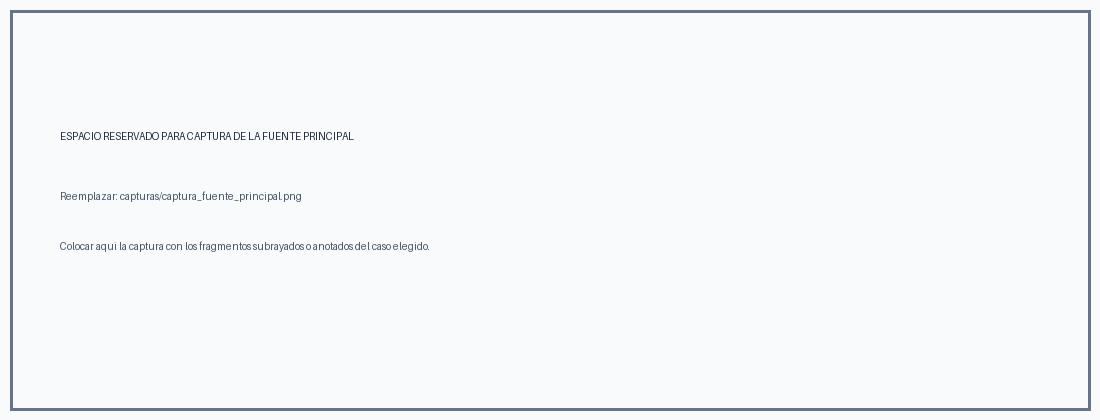
\includegraphics[width=0.92\textwidth]{capturas/captura_fuente_principal.png}
    \caption{Captura de la fuente principal del caso con fragmentos subrayados o anotados \cite{fuente_oficial_caso}.}
    \label{fig:captura_fuente}
\end{figure}

\subsection*{2. Ejemplo de un sistema conocido de primera mano}
\textit{[Describir de autoría propia un sistema que utilices o conozcas de primera mano en el que reconozcas el mismo estilo arquitectónico y justificar por qué.]}

\subsection*{3. Declaración de uso de inteligencia artificial}
\textit{[Indicar de forma explícita y transparente si se utilizó alguna herramienta de inteligencia artificial, en qué etapa se empleó y confirmar la revisión y autoría final del contenido.]}

\clearpage

% ==================== REFERENCIAS ====================
% Verifica manualmente cada DOI en https://doi.org/ antes de entregar.
\printbibliography[title={Referencias}]

\end{document}
